\part{Optimising approximate counterdiabatic driving}\label{part:COLD}

\chapter{Counterdiabatic optimised local driving}\label{chap:4_COLD}

\epigraph{I feel a need… a need for speed.}{LT Pete "Maverick" Mitchell, \emph{Top Gun, 1986}}

In Ch.~\ref{chap:2_adiabaticity} we established that adiabatic evolution of a quantum system requires timescales that scale with the energy gap, without which it experiences non-adiabatic excitations out of its instantaneous eigenstate(s). This presents a problem, as the results of adiabatic dynamics - \@i.e.~the production of the set of adiabatic eigenstates of the final Hamiltonian after the system evolution - is useful in many applications of quantum technologies \cite{dimitrova_many-body_2023, campo_more_2014, ebadi_quantum_2022}, but the timescales this requires are often difficult to achieve due to decoherence and other physical constraints. 

The dual motivation of implementing adiabatic evolution and doing so \emph{fast} has led to the development of a number of methods and approaches under the umbrella of \acrref{STA} \cite{guery-odelin_shortcuts_2019, torrontegui_chapter_2013}, with a universal \acrref{STA} approach being provided by \acrref{CD} \cite{berry_transitionless_2009, demirplak_adiabatic_2003}, introduced in detail in Sec.~\ref{sec:2.3_CD}. However, as established in Sec.~\ref{sec:2.3_CD}, exact \acrref{CD} is often difficult to derive and even more difficult to implement in an experimental setting, leading to the development of approximate methods such as \acrref{LCD} \cite{sels_minimizing_2017} and the truncated nested-commutator approach \cite{claeys_floquet-engineering_2019} which were discussed in detail in Sec.~\ref{sec:2.4.1_LCD} and Sec.~\ref{sec:2.4.2_nested_commutators} respectively. Apart from the already mentioned techniques, many other approaches \cite{saberi_adiabatic_2014, campbell_shortcut_2015, whitty_quantum_2020} have been developed which aim to bypass the inherent complexity of the exact \acrref{CD}, either in the case of small systems or ones which have scaling transformations \cite{del_campo_shortcuts_2013, deffner_classical_2014, deng_superadiabatic_2018}. These approximate methods all have their advantages and drawbacks when applied to particular adiabatic processes, owing both to their approximate nature and the practical aspects of their implementation.  

In this chapter we will present a new method for speeding up adiabatic processes: Counterdiabatic Optimised Local Driving (\acrref{COLD}), which was first developed with the goal of improving upon the results of \acrref{LCD} while retaining the advantages that it offers. Namely: \acrref{COLD} is a method that, given a time-dependent Hamiltonian and a set of physical constraints for the system that is being driven, can be used to construct an approximate counterdiabatic protocol that performs optimally for the given set of constraints on the Hamiltonian and the system. It does this by combining \acrref{LCD} and optimal control, which we explored in detail in Ch.~\ref{chap:3_Quantum_Optimal_control}. While \acrref{LCD} can be used to implement an approximate \acrref{CD} protocol built out of restricted, physically realisable operators, \acrref{COLD} does this via finding an optimal path for the system, such that the approximate counterdiabatic drive is maximally effective in suppressing non-adiabatic effects.

We will begin the chapter by introducing the \acrref{COLD} method in detail. Then, in Sec.~\ref{sec:4.2_COLD_QOCT}, we will explore exactly what part \acrref{QOCT} plays in the new method. This chapter lays the groundwork for the method of \acrref{COLD}, while in Part \ref{part:applications} of the thesis we will present and analyse the results of its numerical implementation in various physical systems.

\section{Counterdiabatic driving and optimal control}\label{sec:4.1_COLD}

Let us begin by explicitly setting the stage for the problem that we want to solve. Given a Hamiltonian $H(\lambda)$, which depends on time via the parameter $\lambda(t)$, and a system prepared in an eigenstate of $H(\lambda_0)$, where $\lambda_0 = \lambda(0)$ (often this is the ground state, but it need not be), our task is to vary the parameter $\lambda$ from its initial value $\lambda_0$ to some final value $\lambda_f = \lambda(\tau)$ during a duration of time $\tau$ such that at the end of the process, the system is in the corresponding eigenstate of $H(\lambda_f)$. More precisely, if \@e.g.~the system starts in the ground state of $H(\lambda_0)$, after the evolution it should be in the ground state of $H(\lambda_f)$. This can be done quite reliably, as per the discussion of Ch.\ref{chap:2_adiabaticity}, as long as the instantaneous eigenstates of the Hamiltonian driving the system are not degenerate throughout the evolution and the driving happens slowly enough (see Sec.~\ref{sec:2.1.2_adiabatic_condition}). However, bearing in mind that such slow evolution is generally not accessible, our primary goal is to achieve this result while keeping $\tau$ small \@i.e.~making the evolution as fast as possible. 

As already mentioned in the introduction to this Chapter, one way to achieve this task is by using \acrref{CD} (Sec.~\ref{sec:2.3_CD}). That is, for a given $H(\lambda)$, it may be possible to derive and implement an exact counterdiabatic Hamiltonian from Eq.~\ref{eq:CD_Hamiltonian} which suppresses all non-adiabatic effects experienced by the system due to fast driving. Exact \acrref{CD} could, in this way, keep a system in the instantaneous eigenstate of $H(\lambda)$ during arbitrarily short driving times (within the geometric speed limit \cite{bukov_geometric_2019}), but exact \acrref{CD} is not generally accessible for an arbitrary Hamiltonian \cite{kolodrubetz_geometry_2017} and often requires highly non-local operators. 

The next best thing to try, then, might be an approximate \acrref{CD} method like \acrref{LCD}. As discussed in Sec.~\ref{sec:2.4.1_LCD}, \acrref{LCD} not only allows one to variationally approximate the full \acrref{CD}, thus suppressing some of the losses associated with non-adiabatic effects, but it also gives one the freedom to choose the basis of operators for the approximation, making it very attractive in experimental settings where only a limited set of physical operators are available. If an ansatz is not forthcoming, it is also possible to use the ideas presented in Sec.~\ref{sec:2.4.2_nested_commutators} to build up a local operator basis which contributes to the full \acrref{CD} via the nested commutator approach \cite{geier_floquet_2021} and to then use the variational method of \acrref{LCD} in order to construct a counterdiabatic schedule made up of a physically implementable subset of that basis. 

The \acrref{LCD} method is powerful, but it is not without its faults. The primary disadvantage of such an approach is that the counterdiabatic drive being implemented will always be an \emph{approximation} unless the ansatz basis is fully representative of the exact \acrref{CD}. In cases where the approximation is a poor one, the \acrref{LCD} technique might not offer any suppression of errors at all. One solution to this would simply be to expand the ansatz basis in order to access more degrees of freedom in describing the \acrref{CD}, but this would be counter to the idea of only requiring a physically implementable set of operators as part of the approximation in order to make it useful in an experimental setting. The other would be to use a different method entirely to achieve the same result by, for example, taking a page out of optimal control theory as covered extensively in Ch.~\ref{chap:3_Quantum_Optimal_control}. It is not obvious, however, that a switch in tactics would lead to an improvement or what the complexity of designing a new approach might be. As discussed earlier, optimal control pulses can be constructed in a multitude of different ways, many of which have structure that may be completely ineffective for suppressing non-adiabatic effects. In the case of more flexible control pulses like \acrref{GRAPE}, which might offer a larger solution space, what we often run into is an issue of efficiency as the number of control parameters increases very quickly. 

This is where we come to the new method, \acrref{COLD}, which was developed with the aim of retaining the advantages of \acrref{LCD} while improving upon its results. The approach begins with the observation that any counterdiabatic schedule will depend on the driving path of the original Hamiltonian for which it is constructed, as discussed extensively in Ch.~\ref{chap:2_adiabaticity}. Namely, if we write a Hamiltonian $H(\lambda)$ as a sum of $N_H$ operators $\{ \mathcal{O}_{\rm H}^{(i)} \}_{i = 1,...,N_H}$ each scaled by a $\lambda$-dependent coefficient $h_i(\lambda) \in \hbb$ (note that we include constant functions here too instead of treating them as time-independent):
\begin{equation}
    H(\lambda, \hbb) = \sum_{i = 1}^{N_H} h_i(\lambda) \mathcal{O}_{\rm H}^{(i)},
\end{equation}
then the \acrref{CD} drive can be expressed as a sum of operators $\{\mathcal{O}_{\rm CD}^{(j)}\}_{j = 1,...,N_{\rm CD}}$ which are scaled by functions $\alpha_{j}(\lambda, \hbb)$ and the rate of change in the parameters $\dotlambda = \frac{d \lambda}{dt}$. That is to say the form of the counterdiabatic drive is a function of the time-dependent parameter $\lambda$, the operators $\mathcal{O}_{\rm H}^{(i)}$ and their $\lambda$-dependent coefficients. Looking back at Eq.~\eqref{eq:CD_Hamiltonian}, we can now write the counterdiabatic Hamiltonian as:
\begin{equation}\label{eq:H_cd_operators}
    \begin{aligned}
        H_{\rm CD} &= H(\lambda, \hbb) + \dotlambda \AGP{\lambda} \\
        &= \sum_{i = 1}^{N_H} h_i(\lambda) \mathcal{O}_{\rm H}^{(i)} + \sum_{j = 1}^{N_{\rm CD}} \dotlambda \alpha_{j}(\lambda, \hbb) \mathcal{O}_{\rm CD}^{(j)},
    \end{aligned}
\end{equation}
where $\{\mathcal{O}_{\rm CD}\}$ is an operator basis of the adiabatic gauge potential $\AGP{\lambda}$ (\acrref{AGP}) which was introduced at length in Sec.~\ref{sec:2.2_AGP}. We can even see how this relationship comes about by looking at the matrix elements of the \acrref{AGP} in Eq.~\eqref{eq:AGP_adiabatic_basis}, which are a function of the instantaneous eigenenergies of $H(\lambda, \hbb)$ and the matrix elements of $\dlambda H(\lambda, \hbb)$, all of which can be written as functons of $\lambda$ and $\hbb$. Note, that in any finite system the operator basis of \acrref{AGP} will be finite.

In this setting, \acrref{LCD} is a way to variationally find the coefficients $\alpha_j$ for a given subset of the full \acrref{AGP} basis $\{\mathcal{O}_{\rm LCD}\} \subset \{\mathcal{O}_{\rm CD}\}$ which minimise the operator distance between the generalised adiabatic force from the exact \acrref{AGP} and the force generated by the approximate \acrref{AGP}. In the case where the ansatz is the full basis set $\{\mathcal{O}_{\rm CD}\}$, one should recover the exact \acrref{AGP} using the variational approach.

The reason for expressing the counterdiabatic Hamiltonian in this way is to make the dependence of the coefficients $\alpha_j$ on the functions $\hbb$ and $\lambda$ explicit. As mentioned at the start of this section, the philosophy of \acrref{COLD} begins with the observation that the form of the counterdiabatic drive will depend on the path of the Hamiltonian in the parameter space of its coefficients, \@i.e.~if we change either $\hbb$ or $\lambda$ (or both), the form of the counterdiabatic drive will change via the functions $\alpha_j$. A different way of looking at it is to view each specific set of parameters $(\hbb, \lambda)$ as defining a new time-dependent Hamiltonian with its own instantaneous eigenbasis that generates different non-adiabatic effects for a finite evolution time (see, \@e.g.~Eq.~\eqref{eq:moving_frame_schrodinger} and the discussion surrounding the \acrref{AGP}).

Let us return to the problem stated at the beginning of this section: our aim is to drive a system which started in an eigenstate of $H(\lambda_0)$ to the corresponding eigenstate of $H(\lambda_f)$ in the shortest amount of time possible. It is important to note that the problem statement does not say anything about the state for any other value of $\lambda$ throughout the evolution, although in the case where exact \acrref{CD} is implemented, the system should follow the instantaneous eigenstates of $H$ throughout the full dynamics. This more relaxed condition means that, as long as the time-dependent Hamiltonian which drives the system matches up with the problem Hamiltonian at the start and end of the dynamics and the system is in the correct eigenstate at those two points, the path that it takes between them is not particularly important barring any other constraints. This observation can now allow us to finally introduce \acrref{COLD}.

\subsection{The method}

In Sec.~\ref{sec:3.2_Quantum_optimal_control}, we delved into the many ways in which driving pulses for quantum systems can be systematically constructed and modified or optimised in order to achieve particular goals. In fact, it is possible to use \acrref{QOCT} to speed up adiabatic protocols too, something that has been studied extensively, with the resulting methods generally grouped under the umbrella of \acrref{STA} \cite{guery-odelin_shortcuts_2019, torrontegui_chapter_2013}. We could imagine casting our original problem of driving a system to a particular eigenstate of $H(\lambda_f)$ as simply an optimisation problem with a cost function focused on state fidelity given by Eq.~\eqref{eq:costfunc_fidelity}. 

In the case of \acrref{COLD}, however, the first step is to construct a control Hamiltonian in the vein of Eq.~\eqref{eq:optimal_control_H} with the constraints that it be equal to $H(\lambda_0)$ at $t=0$ and $H(\lambda_f)$ at $t=\tau$:
\begin{equation}\label{eq:COLD_optimal_control}
    H_{\betabb}(\lambda, \hbb, \betabb) = \sum_{i = 1}^{N_H} h_i(\lambda) \mathcal{O}_H^{(i)} + \sum_{k = 1}^{N_k} \beta_k(\lambda) \mathcal{O}_{\rm opt}^{(k)}.
\end{equation}
Here, $\beta_k(\lambda) \in \betabb$ are the control functions which can be constructed and optimised using the methods described in Sec.~\ref{sec:3.2_Quantum_optimal_control} and $\mathcal{O}_{\rm opt}^{(k)}$ are controllable operators, which can be a subset of $\{\mathcal{O}_{\rm H}\}$ or introduce a new degree of freedom to the Hamiltonian, as long as the constraints that $H_{\betabb}(\lambda_0) = H(\lambda_0)$ and $H_{\betabb}(\lambda_f) = H(\lambda_f)$ are satisfied. 

In the second step of defining \acrref{COLD}, we return to \acrref{LCD} and the observation that our approximate counterdiabatic drive will depend on the coefficients of the Hamiltonian. If we are given an ansatz set of operators $\{\mathcal{O}_{\rm LCD}^{(j)}\}_{j = 1, ..., N_{\rm LCD}}$ and use them to variationally determine the approximate \acrref{CD} protocol for the control Hamiltonian $H_{\betabb}$ of Eq.~\eqref{eq:COLD_optimal_control}, the resulting Hamiltonian will look something like this:
\begin{equation}\label{eq:COLD_Hamiltonian}
    \begin{aligned}
        H_{\rm COLD}(\lambda, \hbb, \betabb) &= H_{\betabb}(\lambda, \hbb, \betabb) + H_{\rm LCD}(\lambda, \hbb, \betabb) \\
        &= \sum_{i = 1}^{N_H} h_i(\lambda) \mathcal{O}_{\rm H}^{(i)} + \sum_{k = 1}^{N_k} \beta_k(\lambda) \mathcal{O}_{\rm opt}^{(k)} + \sum_{j = 1}^{N_{\rm LCD}} \dotlambda \alpha_{j}(\lambda, \hbb, \betabb) \mathcal{O}_{\rm LCD}^{(j)},
    \end{aligned}
\end{equation}
which is the \acrref{COLD} Hamiltonian. 

All that is left now is the third \acrref{COLD} step, which is the optimisation of the coefficients $\beta_k(\lambda)$ using \acrref{QOCT} methods presented in Sec.~\ref{sec:3.2_Quantum_optimal_control}. A natural, though not exclusive, cost function for this process would be the final state fidelity from Eq.~\eqref{eq:costfunc_fidelity} with respect to the desired eigenstate of $H(\lambda_f)$. We will provide a more detailed discussion of the optimal control component of \acrref{COLD} in the next section.

\begin{figure}[t]
    \centering
    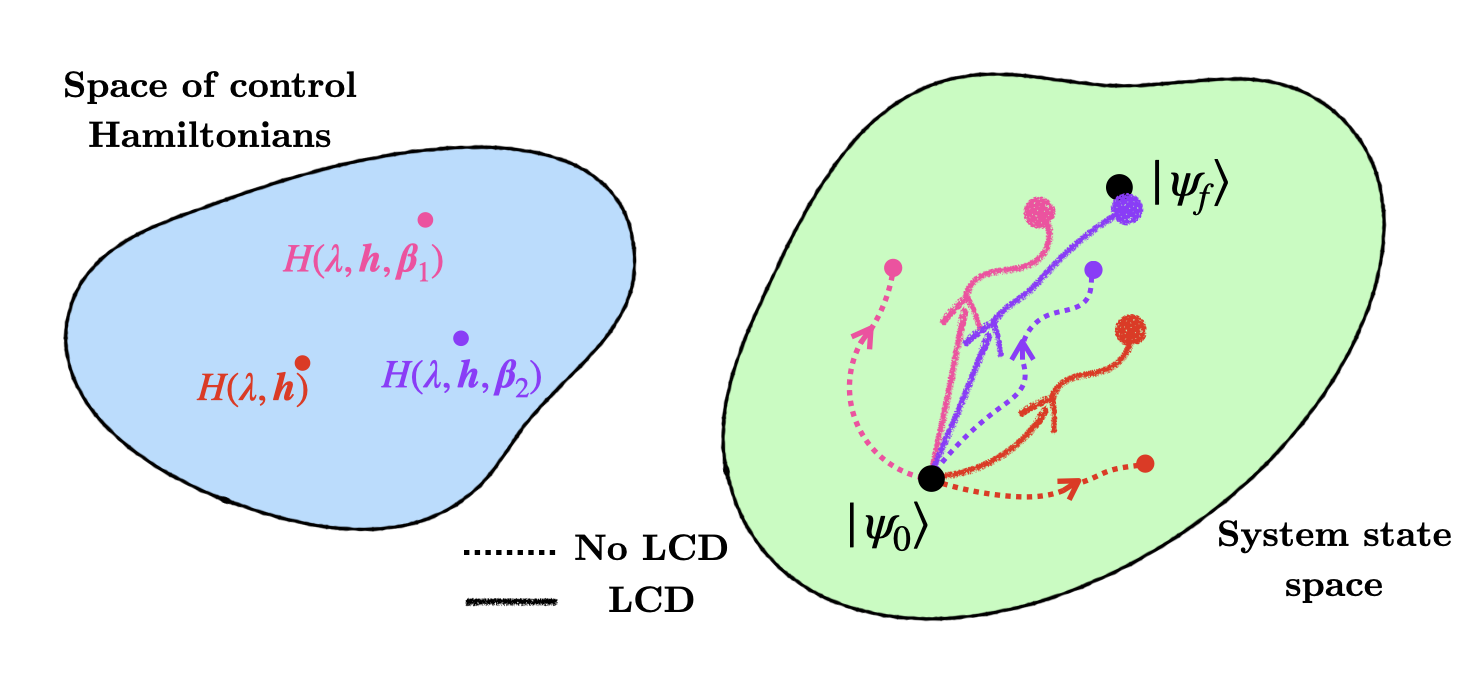
\includegraphics[width=0.8\linewidth]{images/COLD_illustration.png} \caption[A diagrammatic illustration of the COLD method]{A diagrammatic illustration of the COLD method. The blue shape is the set of control Hamiltonians with control parameters $\betabb$, with each point within the shape representing a different instance of $\betabb$. In the case where the control amplitude is $0$ throughout the evolution, we recover the bare Hamiltonian $H(\lambda, \hbb)$ (red point). The green shape represents the system state space with $\ket{\psi_0}$ the eigenstate of $H(\lambda_0)$ that the system is prepared in and $\ket{\psi_f}$ the corresponding eigenstate of $H(\lambda_f)$, which is the target. The dotted (no \acrref{LCD} drive) and chalky (\acrref{LCD} drive included) directed lines show how the system is driven across state space for a fixed total time $\tau$ in the case of each control Hamiltonian indicated on the blue shape. \acrref{COLD} essentially allows one to use optimisation in order to find a path via the value of $\betabb$ which will lead to the result which is closest to the final state when \acrref{LCD} is applied, \@e.g.~going from the red path to the purple.}\label{fig:COLD_illustration}
\end{figure}

The addition of the control pulse prior to applying \acrref{LCD} makes it such that the \acrref{CD} coefficients $\alpha_j$ are now functions of $\betabb$, meaning that varying $\betabb$ will change the shape of the approximate counterdiabatic drive. This is illustrated in Fig.~\ref{fig:COLD_illustration} with changing paths in state space of the driven system. We take the set of operators $\{\mathcal{O}_{\rm LCD}^{(j)}\}$ to be fixed, since in a practical scenario this set would depend on physical constraints of the system for which it is implemented. However, the relative contribution of each operator to the exact counterdiabatic pulse (and thus its effectiveness at suppressing non-adiabatic effects) is governed by the path of the Hamiltonian. By adding a control term, we can now optimise the system evolution to follow a path which allows the truncated counterdiabatic drive to maximally suppress non-adiabatic effects. Fig.~\ref{fig:COLD_illustration} illustrates how the application of \acrref{LCD} will modify any path in system state space to end up closer to the target state than in its absence, but for particular paths it will get much closer. Examples of the effectiveness of \acrref{COLD} in different systems are demonstrated and analysed in more detail in Ch.~\ref{chap:6_Applications_fidelity}, where we explore how \acrref{COLD} holds up against both of its components individually, \acrref{LCD} and \acrref{QOCT}.

\section{Optimal control toolbox}\label{sec:4.2_COLD_QOCT}

With optimal control being one of the two key components of \acrref{COLD}, we will now revisit the content covered in Ch.~\ref{chap:3_Quantum_Optimal_control}, linking it to the way one might go about constructing control pulses in the \acrref{COLD} setting. In Sec.~\ref{sec:3.3_qoct_methods} we covered ``Chopped Randomised Basis" (\acrref{CRAB}) and ``Gradient Ascent Pulse Engineering" (\acrref{GRAPE}), two quantum optimal control methods that offer very flexible yet powerful approaches to constructing and optimising control pulses. Consequently, we can use them in the setting of \acrref{COLD} too. In our original work presented in Ref.~\cite{cepaite_counterdiabatic_2023}, three separate techniques for constructing optimal control pulses were implemented which will be the focal point of Part \ref{part:applications} of the thesis:
\begin{itemize}
    \item `Bare' pulses, which are functions composed of a Fourier basis where each basis function is scaled by an optimisable coefficient, similar to those given by Eq.~\ref{eq:trigonometric_CRAB}. The name `bare' is used to distinguish them from \acrref{CRAB} as they do not include any randomisation component.
    \item COLD-CRAB pulses, which are like the bare version but with the inclusion of randomisation in the frequencies of the basis functions used to construct the pulse, as discussed in Sec.~\ref{sec:3.3.1_CRAB}.
    \item COLD-GRAPE pulses, wherein the optimisable function is constructed using the \acrref{GRAPE} approach of parameterised piecewise constant time slices, as was expanded upon in detail in Sec.~\ref{sec:3.3.2_GRAPE}. 
\end{itemize}

To illustrate, a `bare' pulse, which will make a return often in the next part of the thesis is the function
\begin{equation}\label{eq:bare_pulse}
    f(\lambda, \betabb) = \sum_{k=1}^{N_k} \beta^k \sin (2 \pi k \lambda),
\end{equation}
which fulfills the boundary conditions of $H(\lambda_0)$ and $H(\lambda_f)$ for $\lambda_0 = 0$ and $\lambda_f = 1$. The parameters $\beta_k$ for each frequency $k$ can be optimised using a numerical approach from Sec.~\ref{sec:3.1.3_numerical_optimisation}. This is a very simple way to construct a control pulse, but the simplicity is its appeal: it describes a continuous function with very few parameters and a solution can often be easily analysed once it is found.

The case of COLD-CRAB is more self-explanatory, as it is just an implementation of the \acrref{CRAB} algorithm, which was discussed in detail in Sec.~\ref{sec:3.3.1_CRAB}, to construct the control pulse for \acrref{COLD}. In the numerical results presented in the next part of the thesis, the most common implementation is taking the bare pulse that defined above in Eq.~\eqref{eq:bare_pulse} and randomising the principal frequencies $\omega_k = 2 \pi k$ of the trigonometric functions. This is done by drawing $N_k$ parameters $r_k$ from a uniform random distribution $r_k \in [-0.5,0.5]$ at each optimisation instance of the pulse and replacing $k \rightarrow k(1+r)$. This makes optimisation more complex - as already discussed in Sec.~\ref{sec:3.3.1_CRAB} - but it also often allows for far better results without any increase in optimisable parameters. Depending on the computational resources at hand, especially parallelisation, COLD-CRAB is a far better option than just the bare pulse in terms of results.

Finally, COLD-GRAPE is exactly what it says on the tin - if the tin were Sec.~\ref{sec:3.3.2_GRAPE}. In this case the optimisable pulse is built up out of piecewise constant control amplitudes, as in the original \acrref{GRAPE} algorithm and these are optimised once again using numerical methods from Sec.~\ref{sec:3.1.3_numerical_optimisation}. The method requires far more optimisation parameters and thus is computationally intensive, but it also removed the need to choose a good pulse basis, like in the bare and COLD-CRAB cases. It is possible, but not necessary, to use the gradient information of the cost function that was provided in the original \acrref{GRAPE} paper \cite{khaneja_optimal_2005}. As will become clearer in Ch.~\ref{chap:7_higher_order_agp} however, some of the cost function landscapes we have to deal with in the case of \acrref{COLD} are highly non-convex and as such gradient-based optimisation techniques generally do not work well. 

One computational issue to address in using \acrref{GRAPE} for \acrref{COLD} is that the coefficients $\alpha_j$ of the \acrref{LCD} pulses generally have a dependence on $\dlambda \betabb$ due to the \acrref{AGP} operator being a function of the matrix elements of $\dlambda H$. These are not well-defined for a pulse constructed out of piecewise constant amplitudes masquerading as a continuous function. The way to get around this issue is to use spline interpolation \cite{noauthor_spline_nodate}, which is a method used to interpolate between the piecewise components and recover a continuous pulse which can then be used to calculate the derivatives $\dlambda \betabb$. 

These three methods are by no means the only way to construct optimal pulses for \acrref{COLD} and, as discussed in Sec.~\ref{sec:3.2_Quantum_optimal_control}, the field of quantum optimal control is vast. A consideration that is specific to \acrref{COLD} is the inclusion of constraints in the cost function on the \acrref{LCD} pulse as well as the control drive, as it can diverge \@e.g. across phase transitions \cite{hatomura_controlling_2021}, something that makes experimental implementation difficult and goes against the philosophy of \acrref{COLD} as a method. Ultimately, both the \acrref{LCD} pulse and the control drive should be designed with the goal of making them useful in an experimental setting and the optimal control component needs to reflect this. 